\documentclass[twocolumn]{article}
\usepackage{array,url,kantlipsum}
\usepackage{lmodern}
\usepackage{tikz}
\usepackage{capt-of}
\usepackage{biblatex}
\usepackage{graphicx}

\usetikzlibrary{arrows,decorations.pathmorphing}

\addbibresource{paperdyna.bib}

\tikzset{>=latex}

\tikzset{snake it/.style={decorate, decoration=snake}}

% \Mark is probably provided by spconf, that I don't have
\newcommand{\Mark}[1]{\textsuperscript{#1}}

\begin{document}
\twocolumn[{%
 \centering
 \LARGE Hybrid ARIMA/ANN vs naive model for trading  \\[1.5em]
 \large Repetto Marco\Mark{1},
       \\[1em]
 \normalsize
 \begin{tabular}{*{2}{>{\centering}p{.35\textwidth}}}
  \Mark{1}Dipartimento di Management e Metodi Quantitativi \tabularnewline
  Università degli studi di Milano \tabularnewline
  \url{}marco.repetto@studenti.unimi.it
 \end{tabular}\\[3em] % some more space after the title part
}]

\begin{abstract}
This paper present the combination of an ARIMA process with the neural networks. Such combination is used for signal generation in the prediction of stock prices movement, especially in such case the goodness of such model is tested in comparison with a naive algorithm. The portfolio of such game is built using common stocks from NASDAQ.
\end{abstract}

\section{Introduction}
Trading on securities is probably one of the many field in finance which saw an incredible automatization over recent years and consequently an improvement in efficiency in the markets interested in such innovation\cite{AvellanedaAlgorithmicHighfrequencytrading2011}.

\begin{figure}
    \centering
    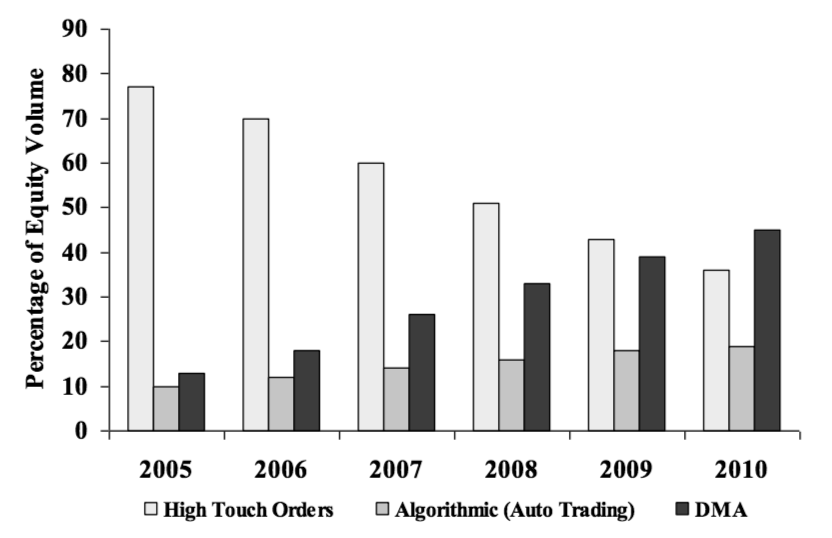
\includegraphics[width=1\linewidth, ]{images/algodata.png}
    \caption{Percentage of order generated by algorithms}
    \label{algodata}
\end{figure}

A completely new professional role came out from such innovation; the Quant, that is, a professional who is expert in quantitative analysis and in particular in financial modelling. The concept of Quant would not be so important without the concept of algorithmic trading, which is defined as automated trading done by computers which are programmed to take certain actions in response to varying market data. In very simplistic and kind of "naive" words the algorithm take the inputs from the model developed by the Quant and enacts the decision supported by the financial model.
In order to let the algorithm implement market decisions (whether to buy or to sell a particular security) we have to "feed" it with a proper financial model. A tipycal algorithmic trading process would is represented on figure \ref{algoproces}; the overall process consists mainly in 4 cyclical phases where two of them interacts comprehend interactions with the environment, as follows:

\begin{itemize}
\item I phase: consists manly on data gathering from the environment $E$, in our case since we are using an univariate time series model our data comes form the sub set $M$ which represent the market data;
\item II phase: at this point the data gathered are used by the quant to create a proper financial model able to forecast the behaviour of the securities under scope; 
\item III phase: this phase embrace the activities of backtesting of the financial model built by the professional;
\item IV phase: eventually the financial moodel is deployed and starts to interact with the market $M$, buying and selling a specific security.
\end{itemize}

In this paper we decided to operate a forecast using a model based on time series, precisely an ARIMA (Auto Regressive Integrated Moving Average) process. Plus following what reported by Tseng et al.\cite{TsengFuzzyARIMAmodel2001} we associated to ARIMA process a neural network setted to capture the behavior of the fitting error of the ARIMA process we built previously.
and we defined an algorithm for pseudo real-time signal generation. Based on such signal the algorithm enact the decision whether to buy a stock (forecasting its increase in price) or sell it (because the price will fall). The overall model has to compete with a "naive" algorithm that perform buy and sell decision based only on the condition that the last price is major than the current one, and sell it when the such price raises.

\begin{center}
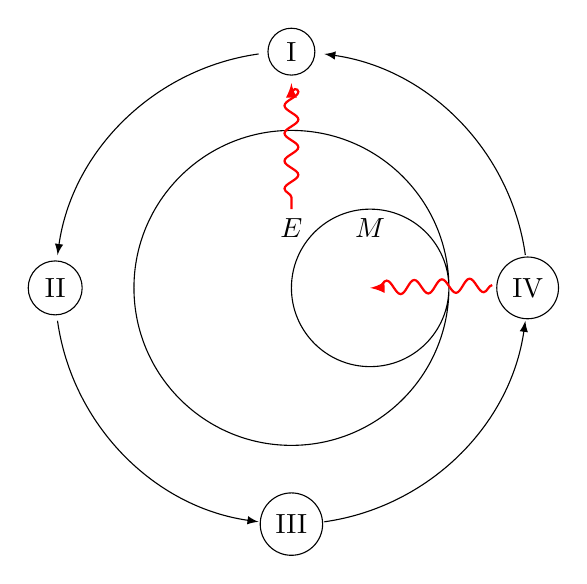
\begin{tikzpicture}

\def \n {4}
\def \radius {3cm}
\def \margin {8} % margin in angles, depends on the radius

  \node[draw, circle] at ({360/\n * (1 - 1)}:\radius) {IV};
  \draw[->, >=latex] ({360/\n * (1 - 1)+\margin}:\radius) 
    arc ({360/\n * (1 - 1)+\margin}:{360/\n * (1)-\margin}:\radius);
    
     \node[draw, circle] at ({360/\n * (2 - 1)}:\radius) {I};
  \draw[->, >=latex] ({360/\n * (2 - 1)+\margin}:\radius) 
    arc ({360/\n * (2 - 1)+\margin}:{360/\n * (2)-\margin}:\radius);
    
     \node[draw, circle] at ({360/\n * (3 - 1)}:\radius) {II};
  \draw[->, >=latex] ({360/\n * (3 - 1)+\margin}:\radius) 
    arc ({360/\n * (3 - 1)+\margin}:{360/\n * (3)-\margin}:\radius);
    
     \node[draw, circle] at ({360/\n * (4 - 1)}:\radius) {III};
  \draw[->, >=latex] ({360/\n * (4 - 1)+\margin}:\radius) 
    arc ({360/\n * (4 - 1)+\margin}:{360/\n * (4)-\margin}:\radius);


\draw (0,0) circle (2) (0,1)  node [text=black,below] {$E$}
      (1,0) circle (1) (1,1)  node [text=black,below] {$M$};
\path [->, thick,draw=red,snake it]
    ({360/5 * (0.9 - 1)+\margin}:2.55) -- (1,0);
\path [<-, thick,draw=red,snake it]
    ({(360/\n * (2 - 1))}:2.6) -- (0,1);
%\draw[draw=blue, snake it] (2,0) arc (0:180:2cm);

\end{tikzpicture}
\end{center}
\captionof{figure}{Algorithmic trading process}
\label{algoproces}
\subsection{AutoRegressive Integrated Moving Average: key concepts and features}
ARIMA process are a class of univariate time series models, this kind of models attempt to predict financial variables using only information contained in their own past values and possibly current and past values of an error term. ARIMA process differ from the exponential smoothing since ARIMA focuses on the autocorrelation of the time series instead of trend and seasonality. Such model firstly proposed by Box-Jenkins\cite{BoxGeorgeTimeSeriesAnalysis} combines three factors, namely: differencing, autoregressive model and moving average model.
\bigbreak
Where differencing is intend as the process of transformation of the timeseries such that we end up with a stationary time series which has as main property no time dependency, in other terms given $X_t$ a stochastic process and $F_X(x_{t_k+\theta})$ its cumulative distribution. $X_t$ is stationary when; $\forall k,\theta and t_k$ we have that:
\[ F_x(x_{t_{k+\theta}}) = F_x(x_{t_k}) \]
Autoregressive models are instead defined as:
\[ c+\phi_1L+...+\phi_pL^p+\epsilon_t \]
In this models we try to forecast future values using a linear combination of past values.
A different appoach is taken by movin average processes, since they do not use past values but instead a regression of the forecast errors.
Moving average models are defined as:
\[c + \theta_1 L + ... + \theta_q L^q)\epsilon_t \]
The concatenation of the three gives us the ARIMA process obtained as:

\begin{equation}
\resizebox{0.9\linewidth}{!}{
$\underbrace{1-\phi_1L-...-\phi_pL^p}_\text{AR(p)} \underbrace{(1-L)^d y_t}_\text{Differencing(d)} \underbrace{c + (1 + \theta_1 L + ... + \theta_q L^q)\epsilon_t}_\text{MA(q)} $}
\end{equation}
\subsection{Artificial Neural Network}
The concept of Artificial Neural Network was firstly proposed by Warren S. McCulloch \cite{mcculloch_logical_1943}.
After a period of stagnation caused by the low processing power of computers at that time, the field saw an incredible expansion in our days and its researching community is one of the most active and perhaps flourish that existed so far.
An Artificial Neural Network is a net based on a series of elements called neurons that are represented by an activation function that given a certain number of input will return an output based on the weights it has.Such activation functions may vary but they are all linear as firstly proposed by B. Widrow \cite{b._widrow_et_al._adaptive_????}.
Fundamental for an artificial neural network is the number of hidden layer that compose such network which may vary from 1 to $n$. In our case we used an artificial neural network with just one hidden layer as proposed by the diagram in figure 3.

\tikzset{%
  every neuron/.style={
    circle,
    draw,
    minimum size=0.5cm
  },
  neuron missing/.style={
    draw=none, 
    scale=4,
    text height=0.333cm,
    execute at begin node=\color{black}$\vdots$
  },
}

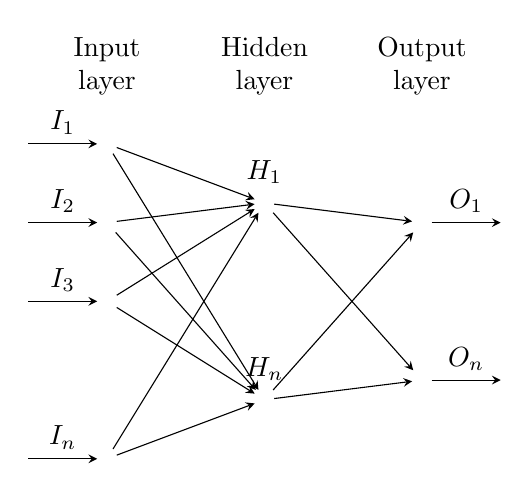
\begin{tikzpicture}[x=1cm, y=1cm, >=stealth]

\foreach \m/\l [count=\y] in {1,2,3,missing,4}
  \node [every neuron/.try, neuron \m/.try] (input-\m) at (0,2.5-\y) {};

\foreach \m [count=\y] in {1,missing,2}
  \node [every neuron/.try, neuron \m/.try ] (hidden-\m) at (2,2-\y*1.25) {};

\foreach \m [count=\y] in {1,missing,2}
  \node [every neuron/.try, neuron \m/.try ] (output-\m) at (4,1.5-\y) {};

\foreach \l [count=\i] in {1,2,3,n}
  \draw [<-] (input-\i) -- ++(-1,0)
    node [above, midway] {$I_\l$};

\foreach \l [count=\i] in {1,n}
  \node [above] at (hidden-\i.north) {$H_\l$};

\foreach \l [count=\i] in {1,n}
  \draw [->] (output-\i) -- ++(1,0)
    node [above, midway] {$O_\l$};

\foreach \i in {1,...,4}
  \foreach \j in {1,...,2}
    \draw [->] (input-\i) -- (hidden-\j);

\foreach \i in {1,...,2}
  \foreach \j in {1,...,2}
    \draw [->] (hidden-\i) -- (output-\j);

\foreach \l [count=\x from 0] in {Input, Hidden, Output}
  \node [align=center, above] at (\x*2,2) {\l \\ layer};

\end{tikzpicture}
\captionof{figure}{Artificial Neural Network scheme}
\label{neural net}

Even though the structure may seem simple one hidden layer ANN reveled to be incredibly reliable on specific task, plus they carry with them greater speed of computation because of its simplicity\cite{the_international_neural_network_society_inns_the_ieee_neural_network_council_cooperating_societies_multi-layer_1990}. As a rule of thumb we take what proposed by Hayashi et al. "Never try a multilayer model for fitting data untill you have tried a single-layer model". Unfortunately there's not such rule of thumb that may help in case of chosing the number of neurons per layer but we choose a number equal two thirds the number of input. 

\subsection{Hybrid ARIMA/ANN process}
The mixed use of ARIMA and neural networks was firstly made by P. Zhang \cite{zhang_time_2003}.
Such process compared to the plain vanilla ARIMA has the advantage of capture features that are not modeled by a univariate process like the ARIMA. In our case we use the neural networks to capture the fitting error behavior of the ARIMA process using the lagged stock price of a bucket of randomly picked stock. In this approach we assume that previous price of the bucket as some kind of power of affecting minimally the future price of the stock or bunch of stock we have.

\section{The empirical study}
The empirical study was made using a portfolio built  with common stock from the NASDAQ. Such portfolio was composed by 30 common stock randomly sampled from the listed company on NASDAQ. From this portfolio we picked a stock and we tested the hibrid ARIMA versus a naive algoritm who generated buy/selling signals at random. We run the game for 30 matches, and every time we retrained our model with the newer informations, leaving aside the older ones.

\subsection{The 30 stocks portfolio}
In order to get the information of the Nasdaq stock we used the API provided by Alphavantage \cite{_alpha_????} and we opted for the 

\section{Evidence and findings}

\section{Conclusion}

\printbibliography

\end{document}